\chapterimage{Pictures/Ausberto/08_Projeto.png}

\chapter{Projeto do Sistema OO}

Um Projeto Orientado a Objetos é um processo por meio do qual um conjunto de modelos de projeto orientados a objetos são construídos pra posteriormente, ser utilizados por programadores para escrever e testar o novo sistema sendo desenvolvido \cite{Satzinger2012}.

\section{Arquitetura do Sistema - Classes}
    O sistema se encontra modularizado e construído através de classes. Todas as páginas visualizadas são compostas por uma ou mais classes.
    
    \begin{itemize}
        \item Arquitetura do sistema completo (Diagrama de Componentes UML)
            Aqui serão mostradas as classes utilizadas por todo o site. Como pode ser visto na enumeração \ref{Classes}, diversas classes foram criadas. Em sua maioria sendo elas páginas ou componentes.
            
            \begin{enumerate}
                \label{Classes}
                \item  TagWholePage
                \begin{enumerate}
                    \item HeaderComponentClass
                    \item HandmadeRouter
                        \begin{enumerate}
                            \item MainPage
                                \begin{enumerate}
                                    \item PageTitle
                                \end{enumerate}
                            \item AddTagPage
                                \begin{enumerate}
                                    \item PageTitle
                                    \item TagCreationHolder
                                \end{enumerate}
                            \item SelfPage
                                \begin{enumerate}
                                    \item PageTitle
                                    \item SelfImage
                                    \item SelfUserContent
                                \end{enumerate}
                            \item AboutPage
                                \begin{enumerate}
                                    \item PageTitle
                                \end{enumerate}
                            \item SignInPage
                                \begin{enumerate}
                                    \item PageTitle
                                    \item UserSignForm
                                \end{enumerate}
                            \item SearchTagPage
                                \begin{enumerate}
                                    \item PageTitle
                                    \item TagTable
                                \end{enumerate}
                        \end{enumerate}
                    \item FooterComponentClass
                \end{enumerate}
            \end{enumerate}
            
        \begin{comment}
            
        \item Arquitetura de um subsistema
            Aqui serão mostradas as classes utilizadas por uma subseção do site. Mais especificamente, a subseção de login.
        \end{comment}
    \end{itemize}

\section{Interfaces do Usuário}
    Em todas as telas teremos sempre o rodapé (footer) e o cabeçalho (header). O footer apenas mostra informações básicas sobre o website. Já o header é onde estão dispostos a logo e o nome do site, assim como também dispõe os botões para navegação entre as diversas páginas do site.
    \begin{itemize}
        \item About

            A página "sobre" (Figura \ref{about}) apresenta as informações referentes ao desenvolvimento do projeto. Seu autor, o responsável, o objetivo e a instituição de ensino.
            \begin{figure}[H]
                \begin{center}
                    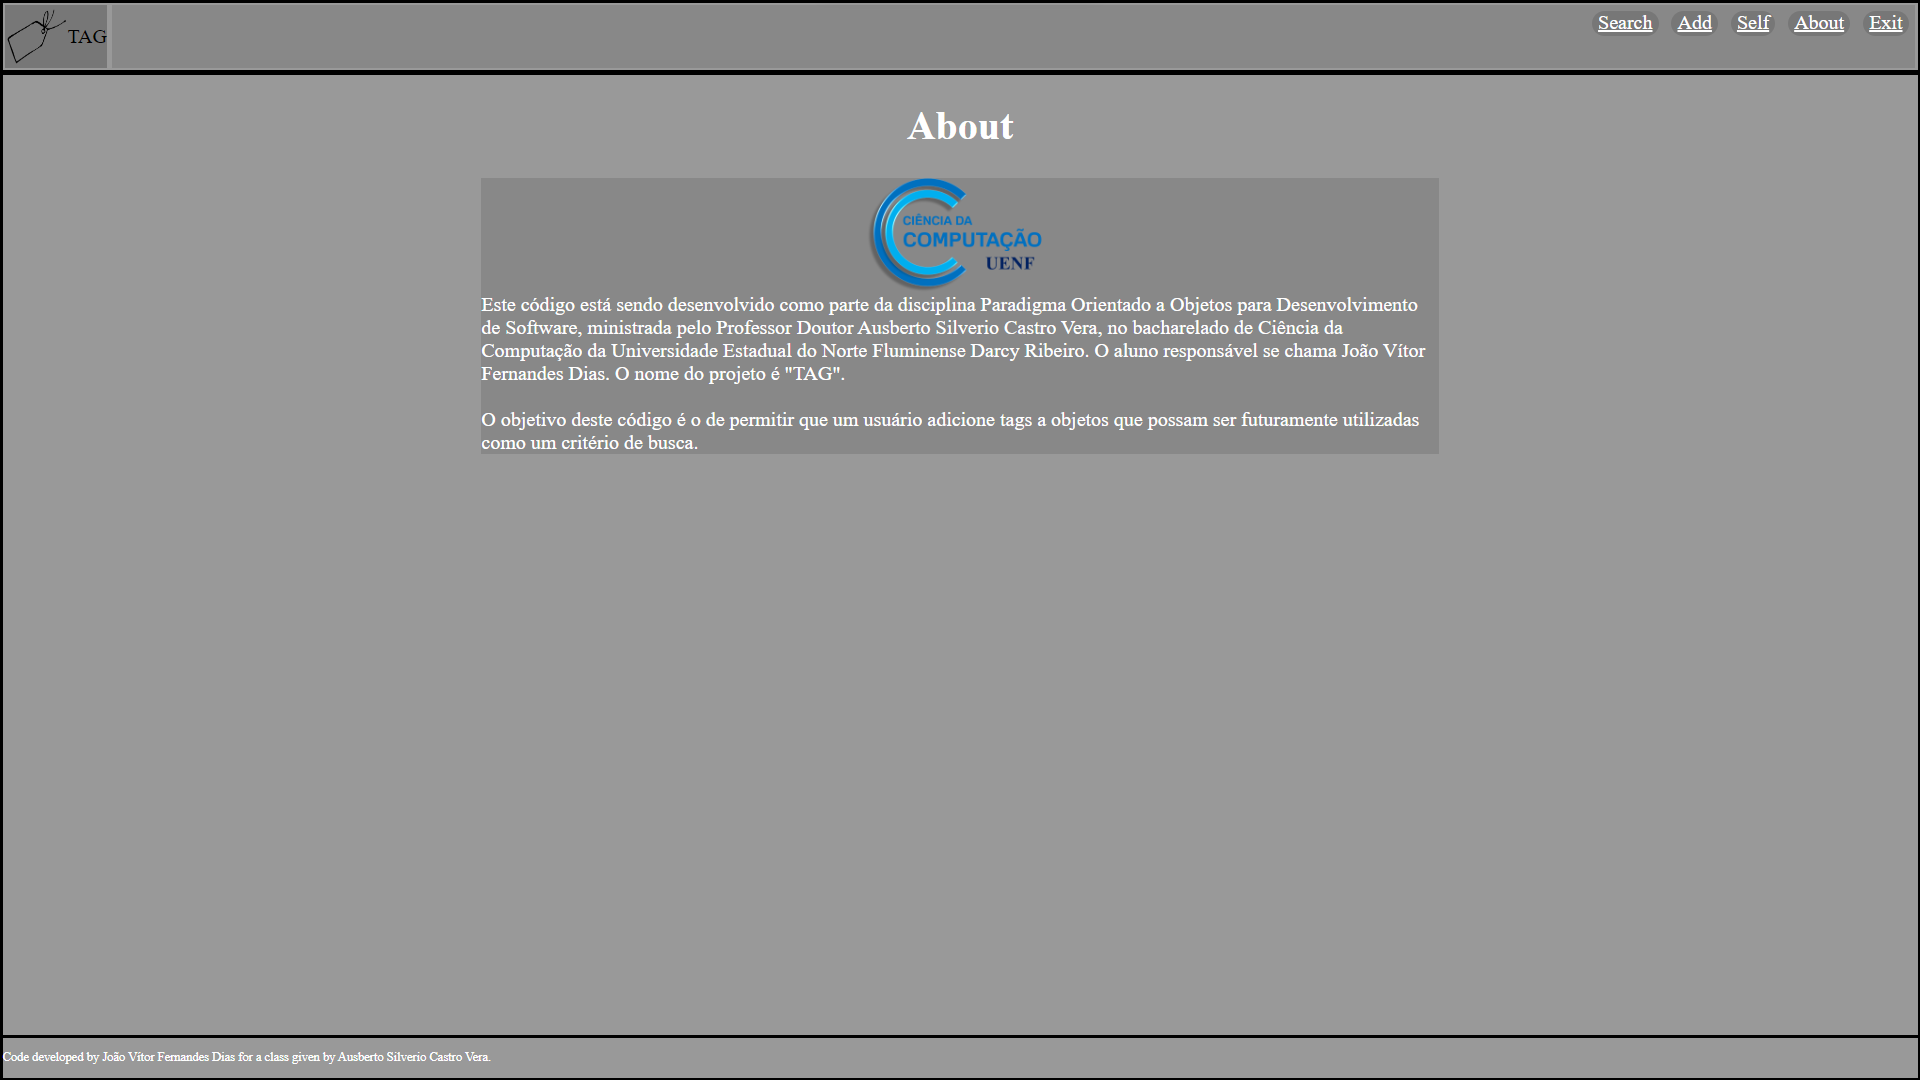
\includegraphics[width=12cm]{Pictures/JV/Interfaces/About.png}
                    \caption{Página Sobre} \label{about}
                \end{center}
            \end{figure}
        \item Search

            Na página de busca (Figura \ref{search}), temos a nossa disposição uma barra de pesquisa para que informemos qual tipo de tag buscamos. Nela podemos digitar qual é a tag desejada, desse modo, logo abaixo serão mostradas as tags correspondentes à pesquisa.
            
            \begin{figure}[H]
                \begin{center}
                    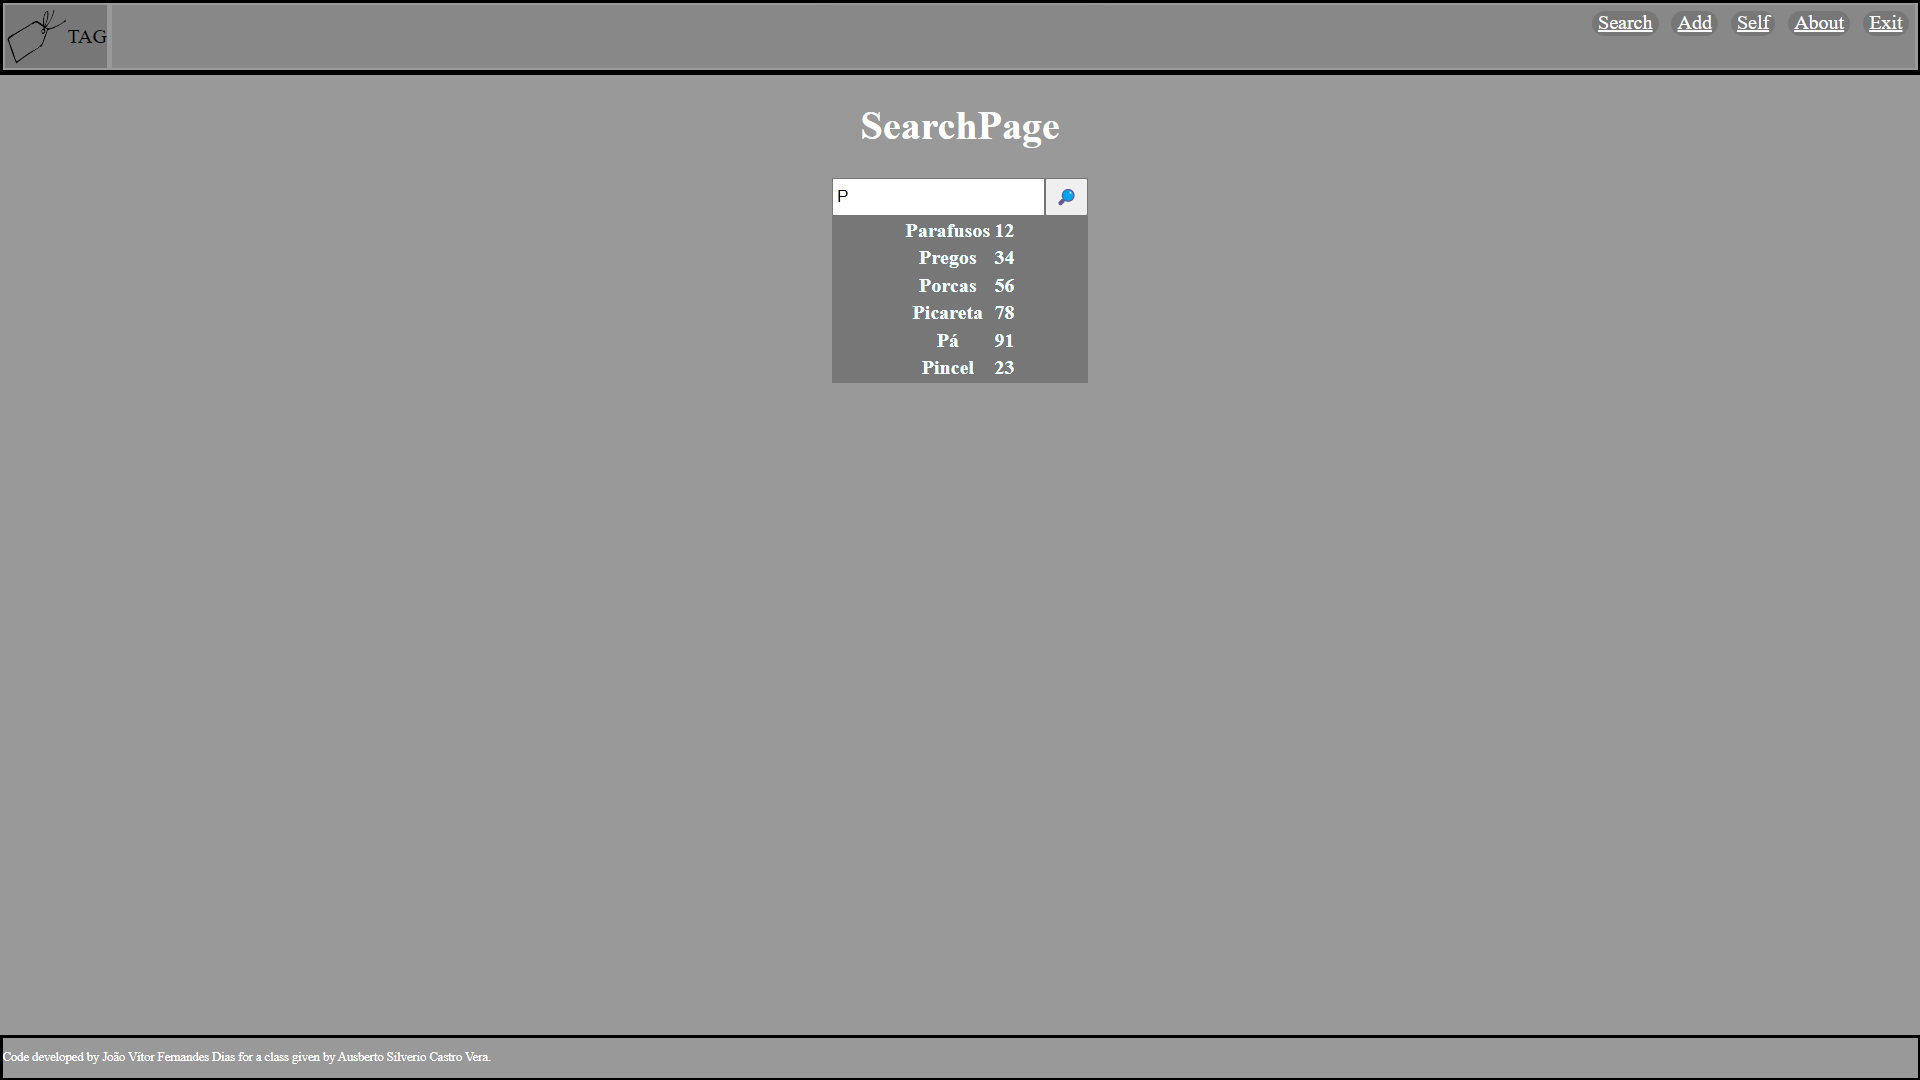
\includegraphics[width=12cm]{Pictures/JV/Interfaces/Search.png}
                    \caption{Página de busca} \label{search}
                \end{center}
            \end{figure}
        \item Self

            Na página do usuário (Figura \ref{self}) são mostradas algumas informações referentes ao usuário, sendo elas o nome do usuário, a senha, seu e-mail, as tags criadas e a data da criação da conta. Também é mostrada a foto de perfil do usuário.
            
            \begin{figure}[H]
                \begin{center}
                    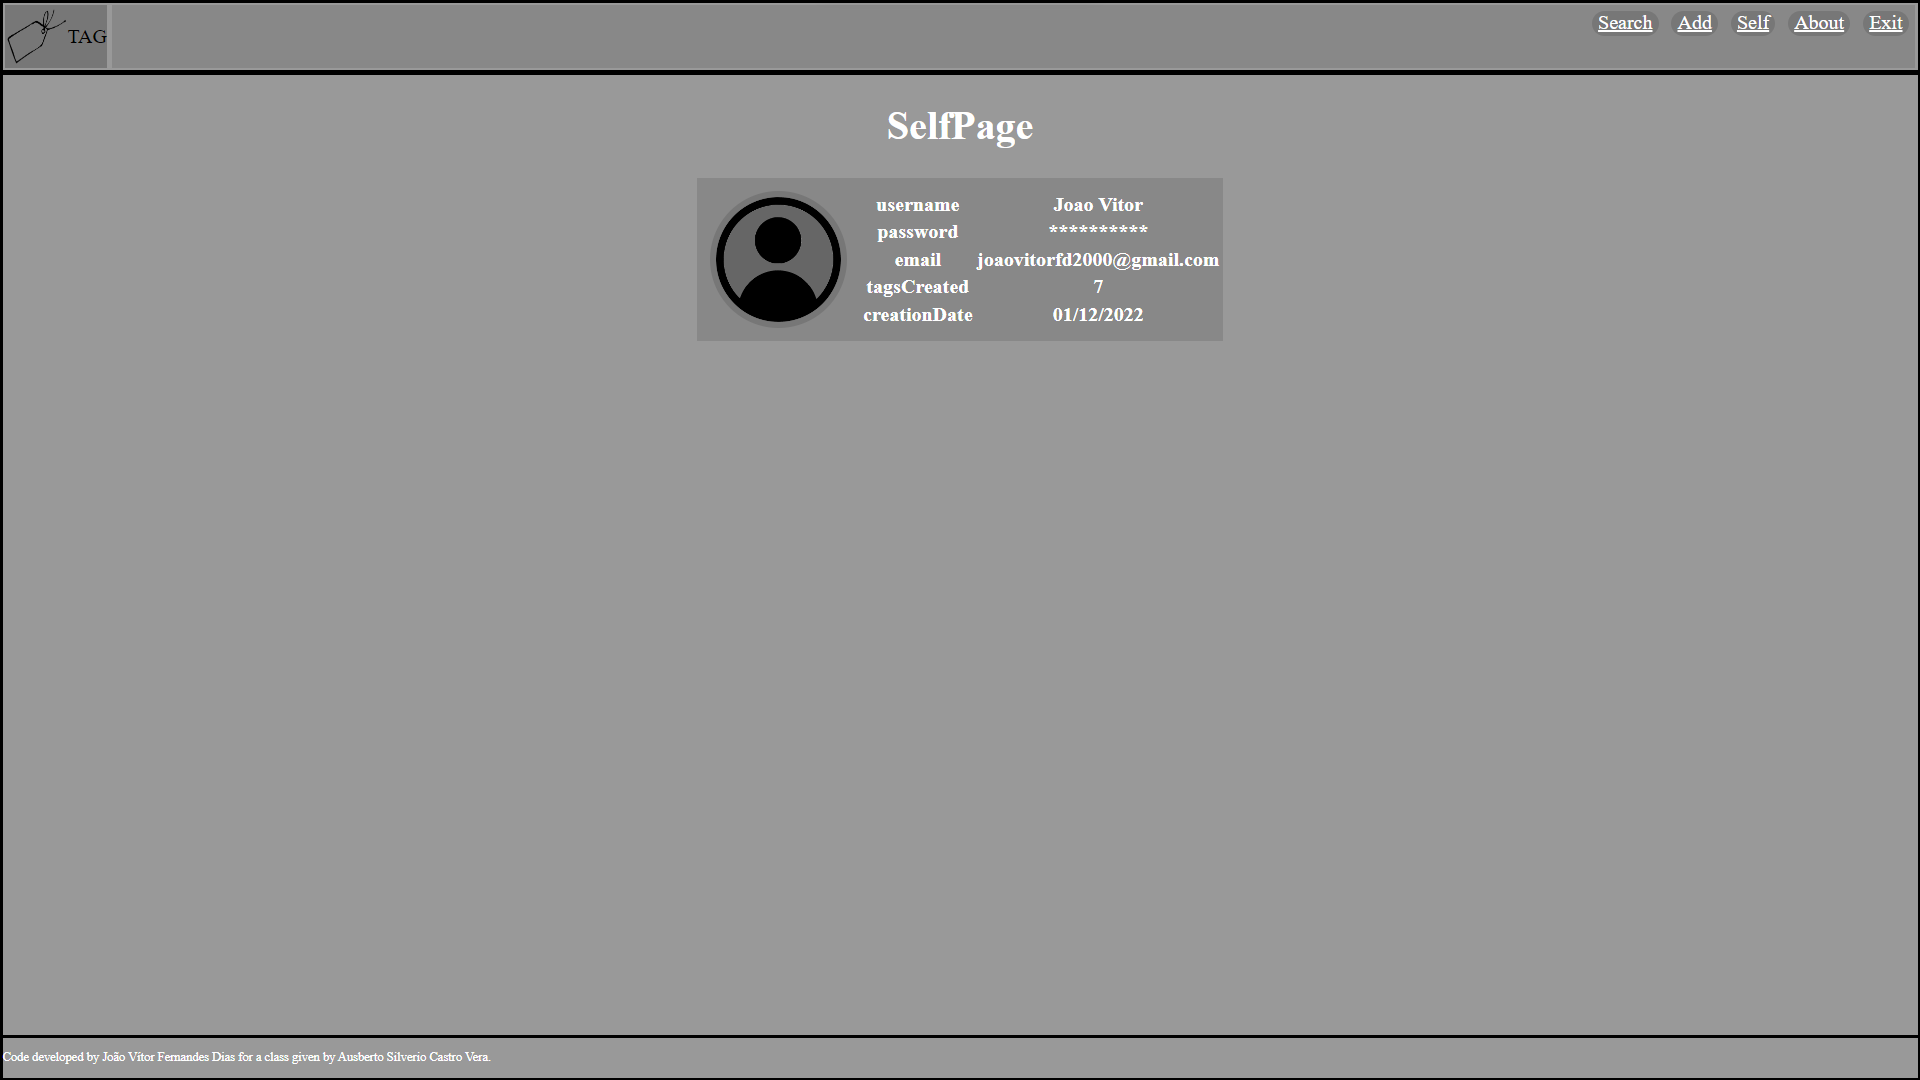
\includegraphics[width=12cm]{Pictures/JV/Interfaces/Self.png}
                    \caption{Página do usuário} \label{self}
                \end{center}
            \end{figure}
        \item SignIn

            Na página de login e cadastro (Figura \ref{sign}), o usuário poderá se conectar ao sistema, ou então se registrar.
                        
            \begin{figure}[H]
                \begin{center}
                    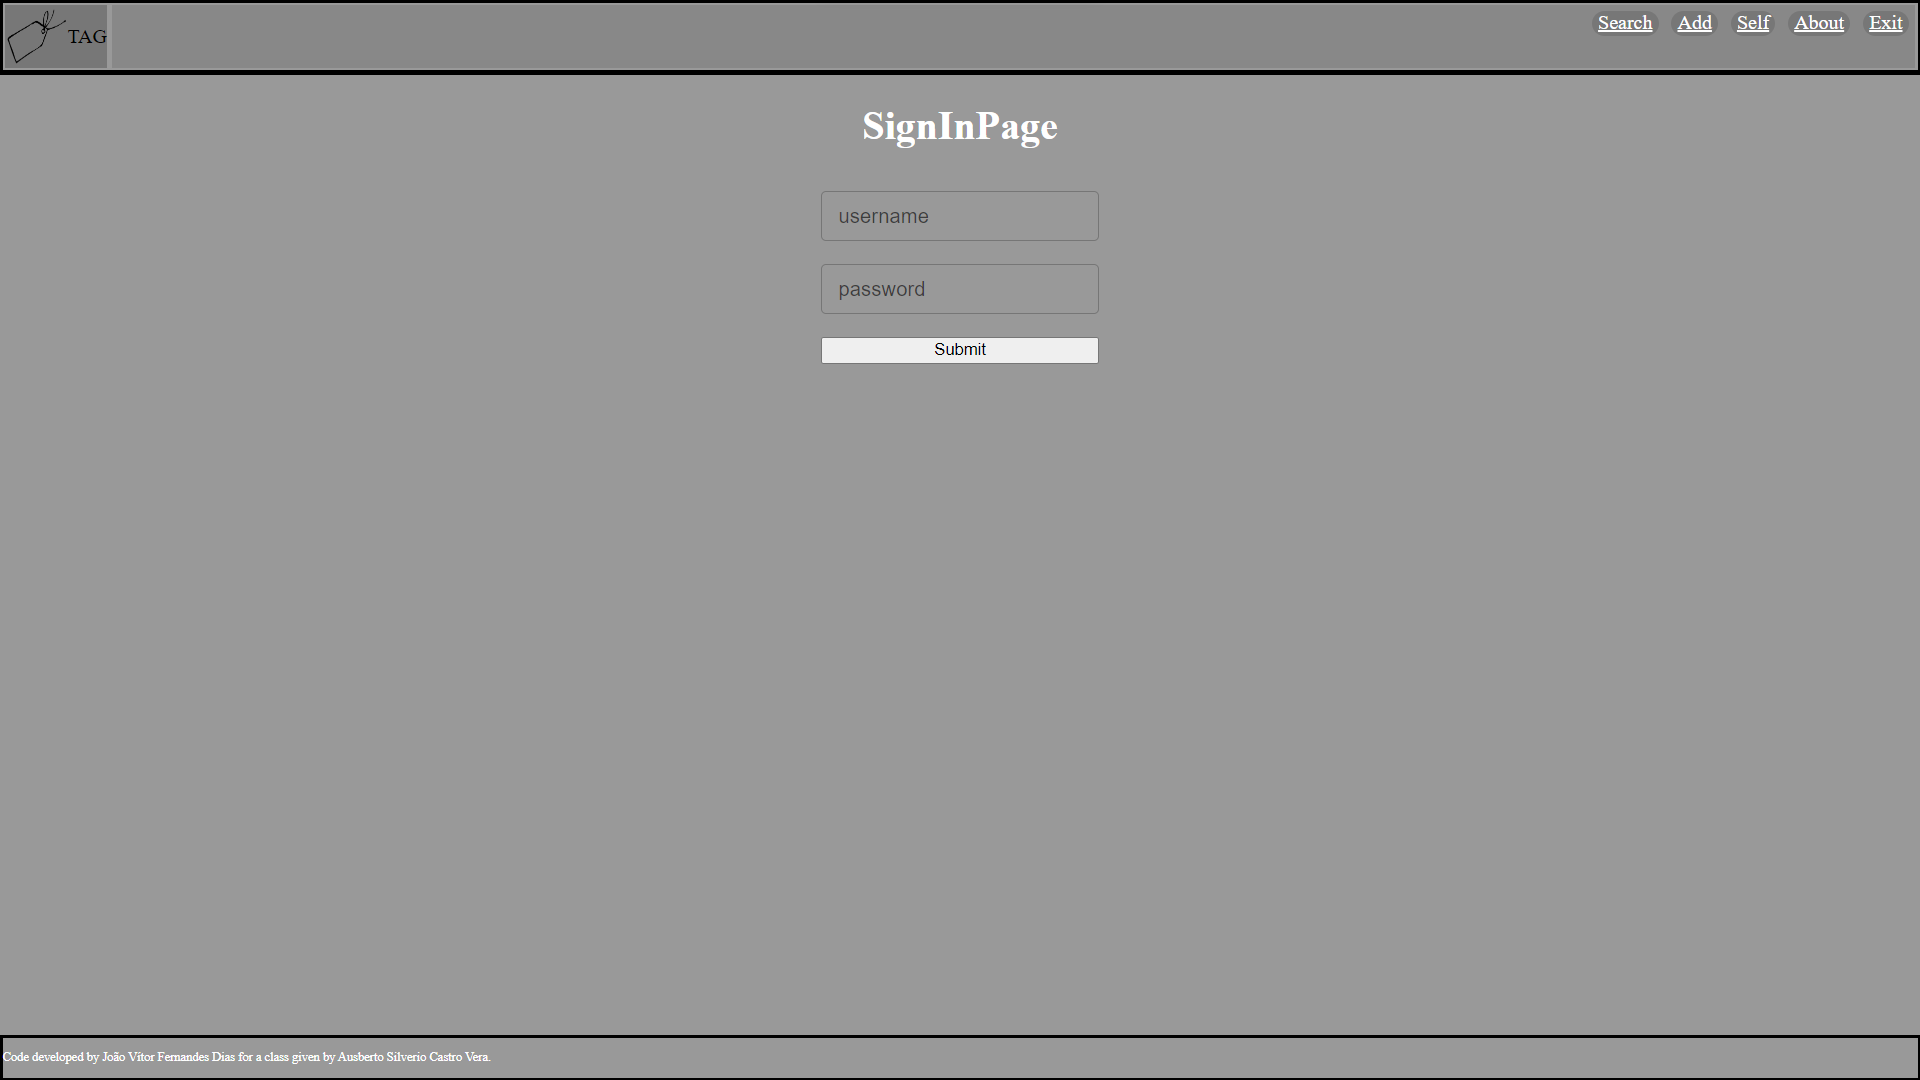
\includegraphics[width=12cm]{Pictures/JV/Interfaces/Sign.png}
                    \caption{Página de login e cadastro} \label{sign}
                \end{center}
            \end{figure}
        \item Tag
        
            Nesta página (Figura \ref{tag}) existem dois campos de texto. O primeiro é referente à chave, já o segundo refere-se ao valor. Há também o botão para registrar a tag correspondente.
            \begin{figure}[H]
                \begin{center}
                    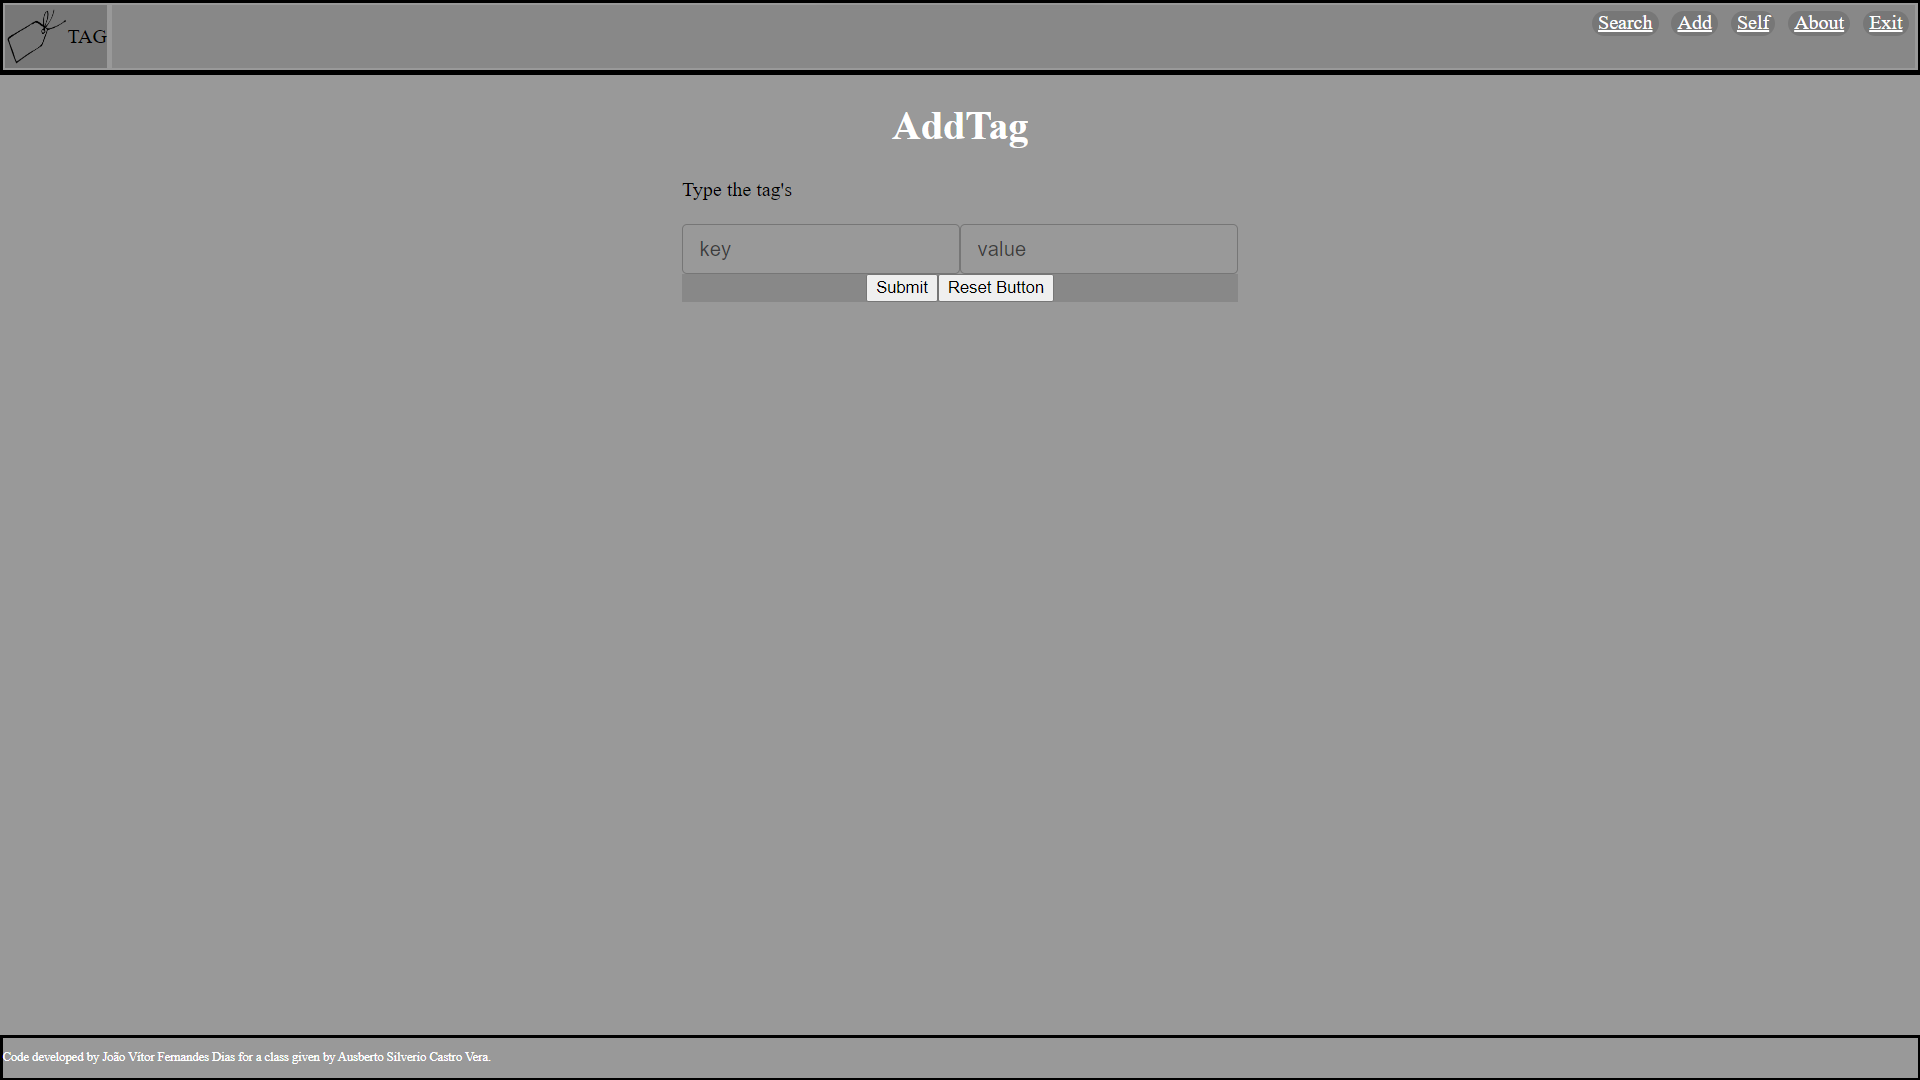
\includegraphics[width=12cm]{Pictures/JV/Interfaces/Tag.png}
                    \caption{Página de adição de tags} \label{tag}
                \end{center}
            \end{figure}
    \end{itemize}

\section{Tabelas de Dados}

    Os dados utilizados pelo website estão todos armazenados em objetos javascript, similares a JSON. Mostrados nas figuras \ref{code7} e \ref{code8}. A primeira faz referência ao armazenamento das tags, já a segunda faz referência ao armazenamento das contas de usuário.

    Dois locais em que essas tags seriam utilizadas mas que não foram implementados são a página Search \ref{Code3} e a página Self \ref{Code4}, visto que a primeira mostraria a pesquisa das tags, enquanto a segunda representa todos os dados do usuário.

\begin{comment}
    Prof. Dr. Ausberto S. Castro Vera
    UENF - CCT - LCMAT - Curso de Ciência da Computação
    Campos, RJ, 2022 
    Disciplina: Paradigma de Desenvolvimento Orientado a Objetos
    Aluno: João Vítor Fernandes Dias
\end{comment}